\documentclass{webofc}
\usepackage[varg]{txfonts}   % Web of Conferences font

\usepackage{float}
\usepackage[caption = false]{subfig}
\usepackage{textcomp}
%\usepackage[final]{graphicx}

\begin{document}

\title{Trident : An Automated System Tool for \\Collecting and Analyzing Performance Counters}

\author{\firstname{Servesh} \lastname{Muralidharan}\inst{1}\fnsep\thanks{\email{servesh.muralidharan@cern.ch}} \and
        \firstname{David} \lastname{Smith}\inst{1}\fnsep\thanks{\email{david.smith@cern.ch}}
}

\institute{CERN, 1211 Geneva CH}

\abstract{%
Trident, a qualitative analysis tool that can look at various low level metrics with respect to the Core, Memory and I/O to highlight performance bottlenecks during the execution of an application. Trident uses a three pronged approach in analysing a node's utilisation of hardware resources and to help a non system expert understand the stress on different parts of the system by a given job. Currently metrics such as memory bandwidth, core utilization, active processor cycles, etc., are being collected. Interpretation of the data in raw form is often non intuitive. Therefore, the tool converts these data into derived metrics that are then represented as a system wide extended Top-Down analysis that helps developers and site managers likewise understand the application behavior without the need for in-depth expertise of architecture details.
}
%
\maketitle
%
\section{Motivation}
\label{sec:moti}

Application performance can be characterized by a myriad of tools and techniques. Some of them rely on hardware and software performance counters of a given system to analyze performance bottlenecks. These counters can come from performance monitoring units (PMUs) built into modern processors, memory controllers, etc., or from software counters present in the underlying operating system. The sheer variety of these counters makes it difficult to quickly narrow down to those associated with a particular performance bottleneck. To tackle this, an approach called Top-Down analysis~\cite{6844459} was developed at Intel based on the counters from Intel processor's PMU. In several cases it was shown that this technique could be used to reliably identify inefficiencies in different areas of a processor that arise from an application.

The effectiveness of Top-Down analysis lies in the fast diagnosis of performance bottlenecks by investigating the derived metrics in a hierarchical manner. However, this approach only works once hotspots are identified in regions of code that account for a large percentage of the execution time. After which Top-Down analysis can be applied to determine optimizations that alleviate, if present, the limitations from the different parts of the architecture. 

In most High-Energy Physics (HEP) codes though, hotspot profiling has been shown to be ineffective~\cite{atlasg4perf}. The reason being the sparse compute code that has been spread over several thousands of C++ classes due to the complex nature of the physics algorithms and implementation inefficiencies. Therefore it has become a key challenge to identify where to focus optimization efforts and to estimate the gain that can be achieved by them. In such a scenario the need for a more qualitative profiling tool becomes a necessity in contrast to the classical fine grained profiling approach.

In this paper we propose Trident, a coarse grained profiling tool tailored to the HEP community. It can quickly identify performance bottlenecks during the runtime of an application by monitoring hardware and software counters. These counters are carefully chosen to simultaneously monitor the key performance metrics of core, memory or IO subsystem of a given node. This three pronged approach allows Trident to form a holistic utilization pattern of a given node in a quick and efficient manner. Tuning the interval of the monitoring allows Trident to be used as a node efficiency analysis tool or a more complex application behaviour characterization tool.

\section{Introduction}
\label{sec:intro}

The concept of performance counter monitoring is neither new nor novel, however in real world scenarios plenty of difficulties arise in effectively following this approach. First to reliably collect hardware counters is a challenge. This is because all of the approaches need support from both hardware i.e. presence of the counters, and software i.e. OS level drivers and configuration. Furthermore, security implications also limit the different ways that can be used to obtain these data as an unprivileged user. Even if overcoming all this was possible for a specific system, scaling these to work in a generic way across a large number of systems is challenging due to the vast variety of configurations. From all this it became apparent that the online counter data collection system also had to be light weight, secure and intelligent enough to detect the specific counters supported by the architecture. All of this had to be done in a non-obscure way that does not sacrifice configurability to support a large variety of systems.

Once the ability to effectively collect the counter data was solved, the next challenge was to apply the formulas for several different derived metrics. In addition this offline analysis also had to perform data parsing and validation. Also some of the derived metrics depend on the configuration of the node, i.e. the number of hyper-threaded cores, memory channels, etc. This information had to be passed on for offline analysis from the monitoring subsystem. 

The Trident tool demonstrates the ability to do timeline based extended Top-Down analysis. Data collected from sparsely spread out interdependent instructions is thereby clustered and gives the potential to allow the identification of regions of the code that could be targeted for further profiling through classic tools. In the rest of this paper we will describe the Trident design architecture in section~\ref{sec:design}, the extended Top-Down analysis and results from a benchmark and an example HEP experiment workload in section~\ref{sec:results}.


\section{Design}
\label{sec:design}

Trident is essentially composed of two distinct functional units. One, a lightweight counter aggregation system that runs continuously and two, a complex offline parser to calculate the different derived metrics from the counter data for an extended Top-Down analysis. The counter aggregation system has to be extremely lightweight such that it has negligible overhead on the application being tested. The offline analysis however, is more complex and can take longer to perform the necessary calculations for the various derived metrics. 

An overview of the Trident system design is shown in figure~\ref{fig:design}. The configurator detects the specific processor model and checks if a corresponding event configuration file is present. If it finds it then it generates a parameter list and launches the collector programs. For the version of Trident described in this paper we use two collectors. The first one is based on \textbf{perf} which records the counters that corresponds to the memory and core. The second one is a perl based wrapper that captures IO counters from \textit{ProcFS}~\cite{bovet2005understanding}.

\begin{figure}
  \centering
	\captionsetup{justification=centering}
  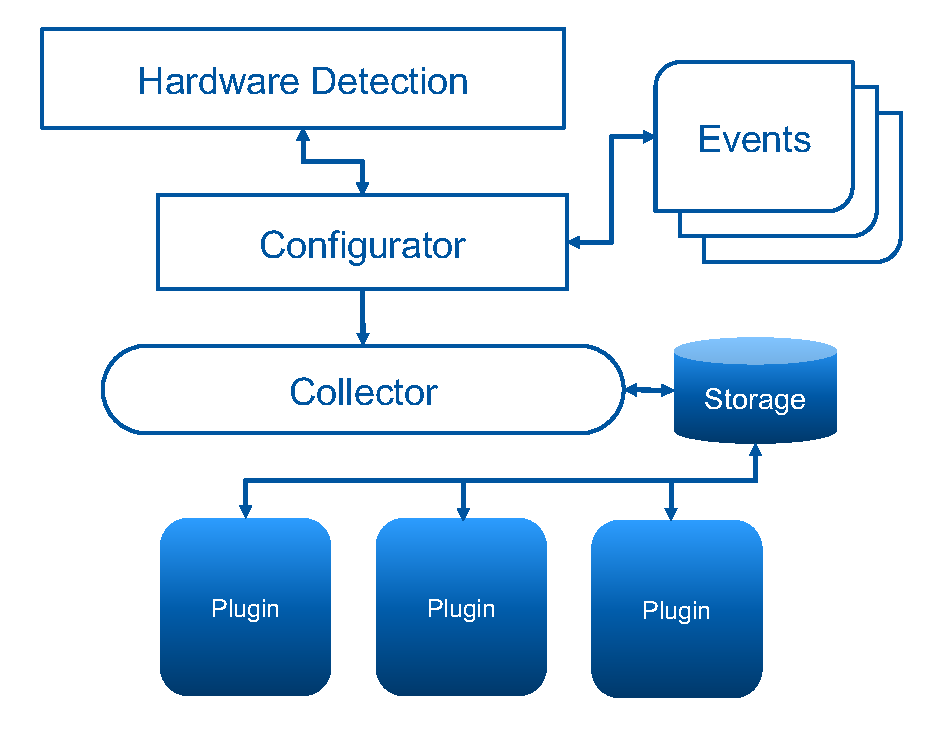
\includegraphics[width=0.5\linewidth]{Design.pdf}
	\setlength{\belowcaptionskip}{-10pt}
\caption{Trident system architecture showing its components and internal design}
\label{fig:design}
\end{figure}

\subsection{Online Measurement}

In order to have little to no influence over the execution of the application, it is essential to collect data from the hardware and software counters with little to no overhead. At the same time the approach has to remain flexible and support systems with little to no software configuration changes. Furthermore for production servers this would need to work without the need for elevated privileges for recording data from the hardware counters. Due to this we were limited to only few choices. 

In order to test the functional idea behind Trident and for the design prototype, the easiest and simplest way to record hardware counters appeared to be piggy backing on the \textbf{perf} subsystem~\cite{perfwiki} of the Linux kernel. After setting up a few simple kernel configuration parameters, it was possible to record counter data from userspace. While \textbf{perf} supports high level counter names, we found this to drastically vary between kernel versions and processors. In addition some of the high level counters that we need do not appear to be directly supported. So therefore we developed a simple architecture identification mechanism using libpfm~\cite{eranian2008perfmon2} and configured a dynamic set of event counters that we validated and tested on a given architecture. The various counters recorded in the current version of Trident is listed in the repository~\cite{tridentrepo}. In the current prototype to aid in debugging and evaluation we write the data to a CSV file~\cite{shafranovich2005common}. However, this is only a limitation of the current system and could be easily remedied by using external monitoring systems such as collectd~\cite{forster2012collectd}.

\subsection{Offline Analysis}
\label{subsec:analysis}

In the current design of the Trident tool a single offline plugin parses the input data file, calculates the derived metrics using preconfigured formulas and generates the necessary graphs that represent the data. We use gnuplot~\cite{janert2010gnuplot} as the underlying graph generator. For further analysis the parsed data is also written to a file in CSV format. The Trident repository~\cite{tridentrepo} lists the various derived metrics we calculate from the recorded counter data.

The data is presented in the form of histograms, one for each type of analysis. This information represents the entire activity of the system recorded at periodic intervals. When an application is executed we can identify the exact time the application is started thereby focus on the period of data that corresponds to this.

\begin{figure}
  \centering
	\captionsetup{justification=centering}
  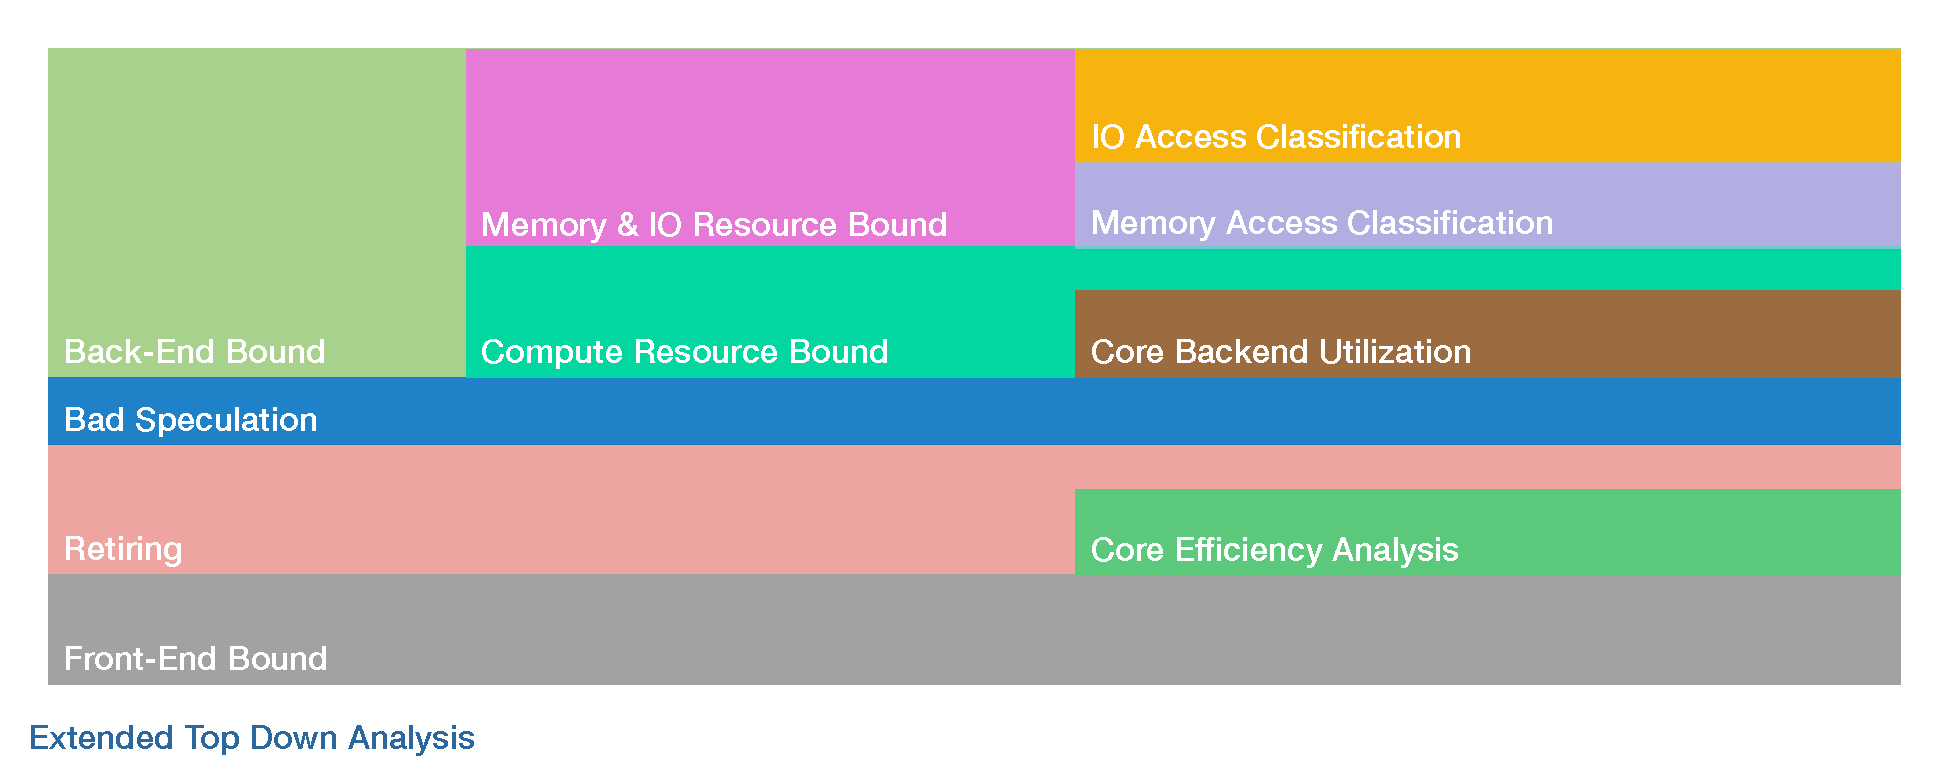
\includegraphics[width=0.7\linewidth]{ExtendedTopDownDiag.pdf}
	\setlength{\belowcaptionskip}{-10pt}
\caption{Extended Top-Down analysis that includes IO and Memory Classification into a single timeline based performance bottleneck identification methodology}
\label{fig:ext_top_down}
\end{figure}

\begin{figure}
  \centering
	\captionsetup{justification=centering}
	\subfloat[Core Efficiency Classification]{\includegraphics[width=0.8\linewidth]{{h06.pmpe16.Trident.1.co}.png}}\\ 
	\subfloat[Core Backend Utilization]{\includegraphics[width=0.8\linewidth]{{h06.pmpe16.Trident.1.cb}.png}}
	\setlength{\belowcaptionskip}{-10pt}
\caption{Core analysis histograms of HEPSPEC06 benchmarks. Each of the benchmark is repeated five times.}
\label{fig:h06-co}
\end{figure}

\begin{figure}
	\centering
	\captionsetup{justification=centering}
	\subfloat[Memory Access Classification]{\includegraphics[width=0.8\linewidth]{{h06.pmpe16.Trident.1.me}.png}}\\
	\subfloat[IO Access Classification]{\includegraphics[width=0.8\linewidth]{{h06.pmpe16.Trident.1.io}.png}}
	\setlength{\belowcaptionskip}{-10pt}
\caption{Memory and IO Access classification histograms of HEPSPEC06 benchmarks. Each of the benchmark is repeated five times.}
\label{fig:h06-me-io}
\end{figure}

\begin{figure}
  \centering
	\captionsetup{justification=centering}
	\subfloat[Core Efficiency Classification]{\includegraphics[width=0.8\linewidth]{{cmd2.pmpe16.Trident.1.co}.png}}\\
	\subfloat[Core Backend Utilization]{\includegraphics[width=0.8\linewidth]{{cmd2.pmpe16.Trident.1.cb}.png}}
	\setlength{\belowcaptionskip}{-10pt}
\caption{Core analysis histograms of an example derivation and reconstruction workload.}
\label{fig:wo-co}
\end{figure}

\begin{figure}
	\centering
	\captionsetup{justification=centering}
	\subfloat[Memory Access Classification]{\includegraphics[width=0.8\linewidth]{{cmd2.pmpe16.Trident.1.me}.png}}\\
	\subfloat[IO Access Classification]{\includegraphics[width=0.8\linewidth]{{cmd2.pmpe16.Trident.1.io}.png}}
	\setlength{\belowcaptionskip}{-10pt}
\caption{Memory and IO Access classification histograms of an example derivation and reconstruction workload.}
\label{fig:wo-me-io}
\end{figure}

Describing the entire Top-Down analysis~\cite{6844459} is beyond the scope of this paper. In figure~\ref{fig:ext_top_down} we show how the generated graphs can be interpreted by the end user to identify bottlenecks in the application being evaluated. We start with core efficiency classification graph to first determine the amount of active CPU cycles and the corresponding IPC ratio during these periods. This tells how busy the core was and how efficiently it could execute the instructions respectively. Then we can narrow down to interesting regions of the program execution and look at how the execution slots were split among Front-End, Back-End, Bad speculation and Retiring. Retiring corresponds to the successful completion of instruction execution. Bad speculation is when the \textmu-op was issued but was never retired due to the need to revert speculative execution. When a \textmu-op was never issued due to a Back-End stall then it is Back-End bound else Front-End bound. If we find that the execution slots were predominantly Back-End bound then this could be due to either the particular Back-End resource was busy or there is wait on the memory or the IO subsystem.

We could then look at the core backend utilization graph to see the specific ports that were busy. If those corresponding to arithmetic operations were most busy then it is most likely that the numerical capability of the processor is at its limit. In case memory operation related ports are busy then the application is either bound accessing large data sets or limited by memory related operations. To investigate further we can look at the memory access classification graph.

If the application is indeed accessing large amounts of data we should see high memory bandwidth during these periods of activity. In this case we can look at the transaction analysis to see if the way data being accessed is limiting performance. e.g., if there were many page misses this could indicate poor memory layout. If instead there was mostly page empty activity accompanied with very low bandwidth to the memory then it could mean very sparse and random access to the data. 

Finally, IO access classification graphs shows the activity the of the disks, SSDs, etc., in the system. If at any point during the execution of the application we notice a period of high IO activity coupled with low core efficiency this could indicate the workload was IO bound. IO access classification can be further represented by either the operation or transfer rate. The amount of data read or written per second is represented by the transfer rate analysis and may be limited by the bandwidth of the disk subsystem. Whereas unique operations are represented by the operation rate analysis and may be sensitive to the latency of the IO subsystem. Of course both can also be influenced by the demands of the application as well as the storage device's technology (hard disk or otherwise) and the connection interface in use. We also represent the peak utilization of the most utilized disk as an indicator of the stress levels of IO activity.

\section{Experimental Results}
\label{sec:results}

To evaluate our Trident tool and to see its usability in real world scenarios we compared the data collected from a known set of benchmarks and a HEP experiment's sample workload. The benchmarks are repeated five times to showcase the ability of the tool to capture and represent data consistently. The sample HEP workload consists of the reconstruction and the derivation of analysis specific formats for a set of events of one of the LHC experiments.

The HEPSPEC06~\cite{michelotto2010comparison}, based on SPEC2006, consists of six individual benchmarks and is used to evaluate and compare compute systems. In figure~\ref{fig:h06-co} we show the core analysis of the various benchmarks and their iterations. It can be clearly seen that each benchmarks stresses different parts of the system as expected. We can see that one benchmark is able to achieve 3 IPC and the corresponding core backend utilization shows the heaviest use of the ports. Most of the benchmarks are also stressing the arithmetic ports indicated by the shades of green in the core backend utilization graph.

In figure~\ref{fig:h06-me-io} we see some of the benchmarks heavily stressing the memory subsystem and in some cases achieves the limit the system is capable of. We can also see that transaction analysis gives a different insight into the way memory is accessed. The IO access classification graphs show very little activity which is representative of benchmark workloads which are designed around compute kernels and do not depend on large data sets.

Similarly in figure~\ref{fig:wo-co} \&~\ref{fig:wo-me-io} we present the information collected during the example workload runs. In contrary to synthetic benchmarks we see a much lower IPC coupled with significant front-end and bad speculation. We can also see four stages in the application execution. While we see heavy usage of the memory operation ports in comparison to the synthetic benchmarks much less access to main memory. Coupled with the information from the transaction analysis we could interpret that there is very sporadic and random access to data. It can also be seen that while there is some IO activity in bursts this by no means is limiting the performance of the workload.


\section{Conclusion}

The concept of Top-Down analysis has been demonstrated previously and has been shown to be effective to identify performance bottlenecks from hardware counter data. Trident has shown that this analysis can also be used in a qualitative form where instead of directly profiling the code we could instead evaluate the functional parts of an application during its execution. In HEP code base with its vast spread of C++ functions, Trident can provide an alternative approach in identifying hotspots to target for improvement by combining relevant functional blocks that are impacted by a particular aspect of the system. The preliminary results presented in this paper shows that this methodology can be quite effective in evaluating workloads in comparison to known benchmarks.

\bibliography{chep18}

\end{document}
